
\subsection{Pied de support}

\begin{frame}{Proprioception du pied de support (1/2) -- Méthodes}
    \begin{columns}
        \begin{column}{0.4\linewidth}
            \begin{block}{Estimation par le modèle géométrique}
                Pied le plus bas
            \end{block}
            \begin{block}{Estimation par les capteurs de pression}
                Pied mesurant le plus de poids
            \end{block}
            \vspace{1.0em}
            \centering
            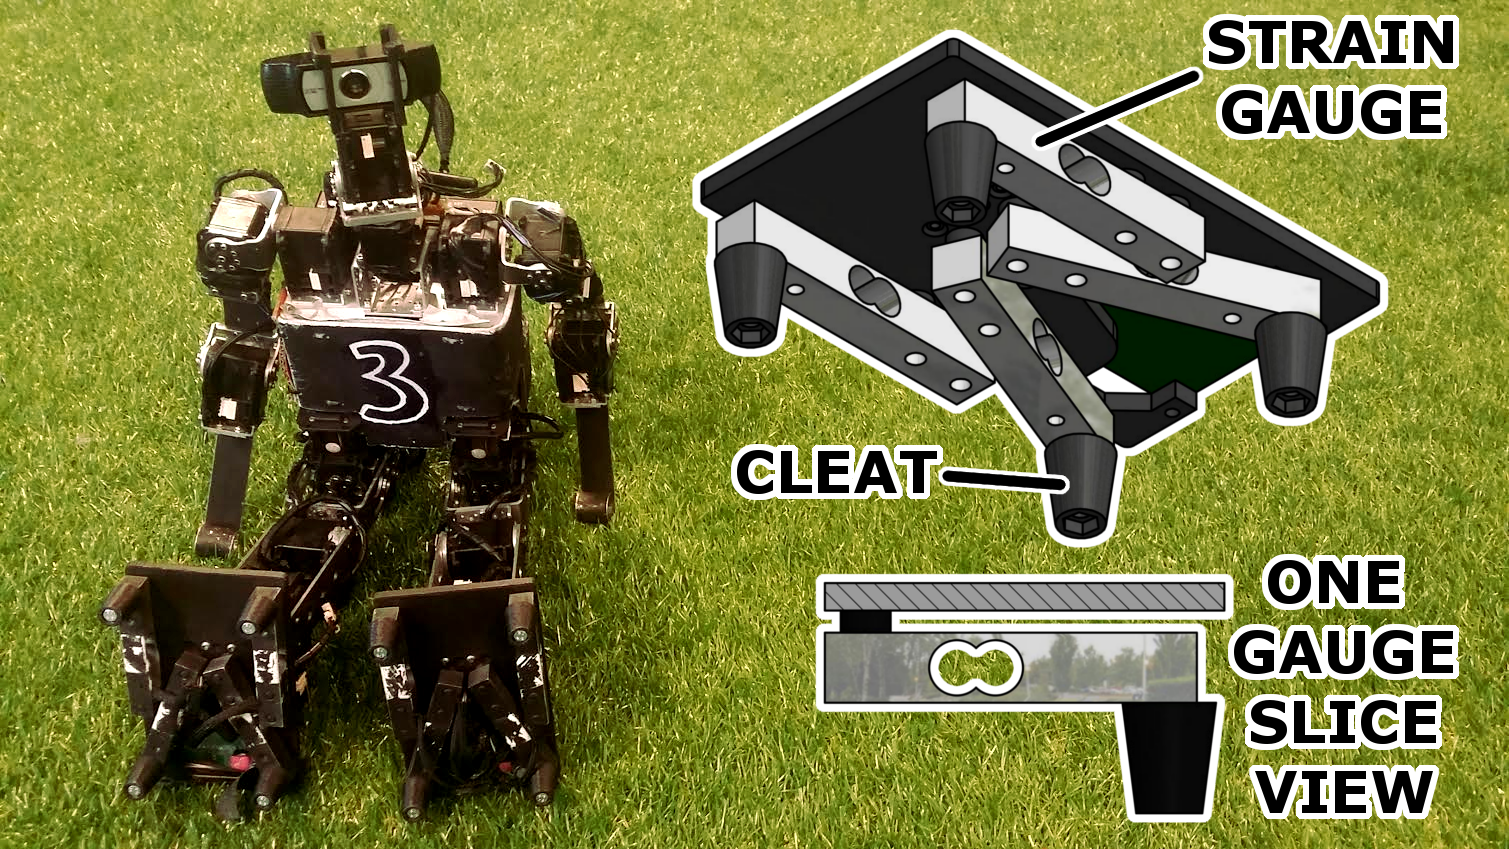
\includegraphics[width=1.0\linewidth]{../media/pressures1.png}
        \end{column}
        \begin{column}{0.6\linewidth}
            \centering
            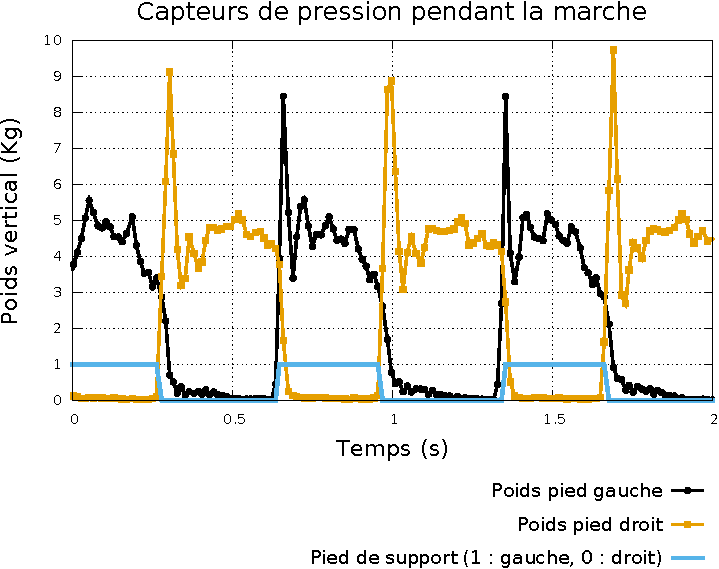
\includegraphics[type=pdf,ext=.pdf,read=.pdf,width=1.0\linewidth]{../plot/pressure_sensors}
        \end{column}
    \end{columns}
\end{frame}

\begin{frame}{Proprioception du pied de support (2/2) -- Comparaison}
    \begin{columns}
        \begin{column}{0.4\linewidth}
            Pilotage manuel. Comparaison de l'odométrie proprioceptive :
            \vspace{1.0em}
            \begin{itemize}
                \setlength\itemsep{1em}
                \item Capteurs de pression > modèle géométrique directe
                \item Dérive de l'azimut
            \end{itemize}
        \end{column}
        \begin{column}{0.6\linewidth}
            \centering
            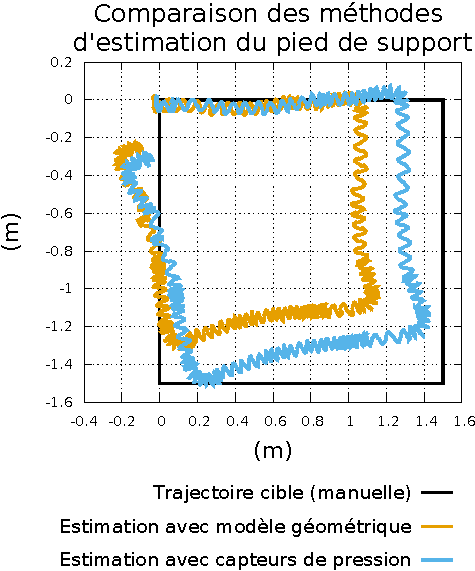
\includegraphics[type=pdf,ext=.pdf,read=.pdf,width=0.75\linewidth]{../plot/odometry_pressure_comparison}
        \end{column}
    \end{columns}
    \begin{block}{}
        \customtextcolor{
            \small
            \textit{Low-cost force sensors for small size humanoid robot}}\\
        \scriptsize
        Grégoire Passault, Quentin Rouxel, Ludovic Hofer, Steve N'Guyen, Olivier Ly\\
        Video contribution, Humanoids, 2015\\
    \end{block}
\end{frame}

\begin{frame}{Imperfections de l'odométrie}
    \begin{columns}
        \begin{column}[T]{0.45\linewidth}
            Erreurs systématiques :
            \begin{itemize}
                \setlength\itemsep{0.5em}
                \item Déformations mécaniques
                \item Latence bas niveau
                \item Filtrage IMU
                \item Erreurs d'asservissement
            \end{itemize}
        \end{column}
        \begin{column}[T]{0.45\linewidth}
            Erreurs non systématiques :
            \begin{itemize}
                \setlength\itemsep{0.5em}
                \item Double support
                \item Glissements (sens de l'herbe)
                \item Collisions entre robots
            \end{itemize}
        \end{column}
    \end{columns}
\end{frame}
